%!TEX encoding=UTF-8 Unicode
\documentclass[xcolor={usenames,dvipsnames}]{beamer}

%=========================Language and encoding ==============================

\usepackage[utf8]{inputenc}
\usepackage[english]{babel} 
\usepackage[T1]{fontenc} 
% Fix size errors due to T1 in bbl file
\usepackage{fix-cm}
%=============================================================================

%========================= Todo notes  =======================================

\usepackage{xkeyval}
\usepackage{todonotes}
\presetkeys{todonotes}{inline}{}

%=============================================================================

%========================= Figures ===========================================

\usepackage{graphicx} % support the \includegraphics command and options
\graphicspath{ {./img/} }
%\usepackage{tikz}
\usepackage{caption}
\usepackage{epstopdf}
%\usepackage{subcaption}

%=============================================================================

%========================= Lstlistings =======================================

%\usepackage{listings}
%
%\lstdefinelanguage{algo}%
%{
%    alsoletter={\\,[,],/,*,\,},%
%    morekeywords=[2]{si, sinon, alors, finSi, pour tout, finPour, tantQue,%
%    finTantQue, ou, et, non, vrai, faux},%
%    otherkeywords={},%
%    morestring=[b]"
%}
%
%
%\lstset{% general command to set parameter(s)
%    basicstyle=\tiny,
%    % print whole listing small
%    keywordstyle=\tiny\color{red}\bfseries,
%    % bold BrickRed keywords
%    %identifierstyle=,
%    % nothing happens
%    commentstyle=\tiny\color{blue}, % blue comments
%    stringstyle=\ttfamily,
%    % typewriter type for strings
%    showstringspaces=false, 
%    numberstyle=\tiny, %size of the fonts that are used for the line-numbers     
%    numbers=left, %num ligne
%    stepnumber=1, %ttes les lignes
%    numbersep=10pt, %decala num ligne/ texte
%    %mathescape=true,%mode math ok
%    tabsize=4, %tabulation
%    frame=single,%encadrement simple
%    frameround=tttt,%encadrement
%    language=algo,
%    morecomment=[s]{/*}{*/},%commentaires speciaux en rouge
%    extendedchars=false,
%    breaklines=true,
%}

%=============================================================================

%========================= Hyperref ========================================== 

\usepackage{hyperref}
\hypersetup{
    dvips,
    backref=true, %permet d'ajouter des liens dans...
    pagebackref=true,%...les bibliographies
    hyperindex=true, %ajoute des liens dans les index.
    colorlinks=false, %colorise les liens
    breaklinks=true, %permet le retour à la ligne dans les liens trop longs
    urlcolor= blue, %couleur des hyperliens
    linkcolor= black, %couleur des liens internes
    bookmarks=true, %créé des signets pour Acrobat
bookmarksopen=true,} 

%=============================================================================

%========================= Other useful includes =============================

\usepackage{amsmath,amssymb} 
\usepackage{array} % for better arrays (eg matrices) in maths
\usepackage{enumerate}
\usepackage{color} %avec un peu de couleur
\usepackage{ifthen}
\usepackage[absolute,overlay]{textpos} %to set som blocks position
%=============================================================================

%========================= Beamer theme =====================================

%Stuff for printable version
\mode<handout>{
    \usetheme{default}
    \setbeamercolor{background canvas}{bg=black!5}
    \pgfpagesuselayout{4 on 1}[letterpaper,landscape,border shrink=2.5mm]
}

%based on Antibe theme
\usetheme{Antibes}

\newcommand{\romannum}[1]{\MakeUppercase{\romannumeral#1}}
\newcommand{\sectnumb}{\romannum{\thesection{}}}

%for white section name
\newcommand{\sectiontitle}{}
\newcommand{\newsection}[1]{\renewcommand{\sectiontitle}{#1}\section{#1}}
\newcommand{\newHsection}[1]{\renewcommand{\sectiontitle}{#1}\section*{#1}}
\newcommand{\subsectiontitle}{}
\newcommand{\newsubsection}[1]{\renewcommand{\subsectiontitle}{#1}\subsection{#1}}



%redifined tree
\setbeamertemplate{headline}
{%
    %title color box
    \begin{beamercolorbox}[wd=\paperwidth,colsep=1.5pt]{upper separation line head}
    \end{beamercolorbox}
    \begin{beamercolorbox}[wd=\paperwidth,ht=2.5ex,dp=1.125ex,%
        leftskip=.3cm,rightskip=.3cm plus1fil]{title in head/foot}
        \usebeamerfont{title in head/foot}\inserttitle
    \end{beamercolorbox}
    %section box
    \begin{beamercolorbox}[wd=\paperwidth,ht=2.5ex,dp=1.125ex,%
        leftskip=.3cm,rightskip=.3cm plus1fil]{section in head/foot}
        \usebeamerfont{section in head/foot}%
        \ifx\insertsectionhead\empty\else%
        %hook
        {\color{white}\hskip2pt\raise1.9pt\hbox{\vrule width0.4pt%
        height1.875ex\vrule width 5pt height0.4pt}\hskip1pt}%
        %section number and section title
        \sectnumb\ \sectiontitle%
        \ifx\insertsubsectionhead\empty\else%
        %end of the tree
        \ \raise1.5pt\hbox{\vrule width 5pt height0.4pt}\ %
        %subsection number and section title
        \thesubsection{}\ \subsectiontitle%
        \fi%
        \fi%
    \end{beamercolorbox}
}

%red color theme
\usecolortheme{beaver}
\useinnertheme[shadow]{rounded}
%structure color (bullets, blocks, table etc.)
\setbeamercolor{structure}{fg=BurntOrange}

% foot line
\definecolor{lightgrey}{RGB}{230 230 230}
\setbeamercolor{footline}{bg=lightgrey, fg=black}
\setbeamertemplate{footline}[text line]{%
    \begin{beamercolorbox}[wd=\paperwidth,ht=2.5ex,dp=1.125ex,%
        leftskip=.3cm,rightskip=.3cm plus1fil]{footline}\insertshortauthor\ %
        (\insertshortinstitute)\hfill\insertframenumber/\inserttotalframenumber%
    \end{beamercolorbox}
}
%=============================================================================

%========================= Title frame  ======================================
\title[]{Analysing a complex scientific application}
%\subtitle{Parallelization and scheduling schemes within SOFA}
\author[Beniamine David]{Beniamine David\\ Under the supervision of \\
Guillaume Huard \and Bruno Raffin}
%\institute[MOAIS]{Univ. Grenoble alpes, Lig - Inria team MOAIS} 
\institute[MOAIS]{
        
\includegraphics[width=.32\textwidth]{img/logoUJF.jpg}
        \qquad
        \qquad
        
\includegraphics[width=.15\textwidth]{img/LIG_coul.jpg}
        \\
        
\includegraphics[width=.22\textwidth]{img/inria.jpg}
        
\includegraphics[width=.4\textwidth]{img/moais.png}
} 
%=============================================================================

\begin{document}
%========================= Title and outlines ================================
\begin{frame}{ }
    \titlepage
\end{frame}

\newboolean{sectiontoc}
\setboolean{sectiontoc}{true} % default to true

\AtBeginSection[]
{
    \ifthenelse{\boolean{sectiontoc}}{
        \begin{frame}<beamer>
            \frametitle{Outline}
            \tableofcontents[currentsection,currentsubsection]
        \end{frame}
    }
}
\AtBeginSubsection[]
{
    \ifthenelse{\boolean{sectiontoc}}{
        \begin{frame}<beamer>
            \frametitle{Outline}
            \tableofcontents[currentsection,currentsubsection]
        \end{frame}
    }
}

%=============================================================================

%========================= Real presentation =================================
\begin{frame}{Outline}
    \tableofcontents 
\end{frame}

\newsection{Context and motivations}

\begin{frame}{Context}
    \begin{block}{Physical simulation}
        \hfill
        \parbox[c][.26\textheight][t]{.98\textwidth}{
                %\only<1>{\input{img/simulation_pipeline0.tex}}
                %\only<2>{\input{img/simulation_pipeline1.tex}}
            \only<1>{ 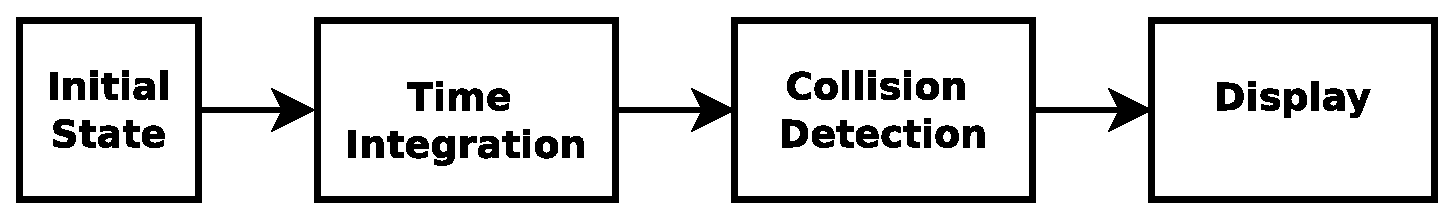
\includegraphics[width=.95\textwidth]{simulation_pipeline2.eps}}
            \only<2>{ 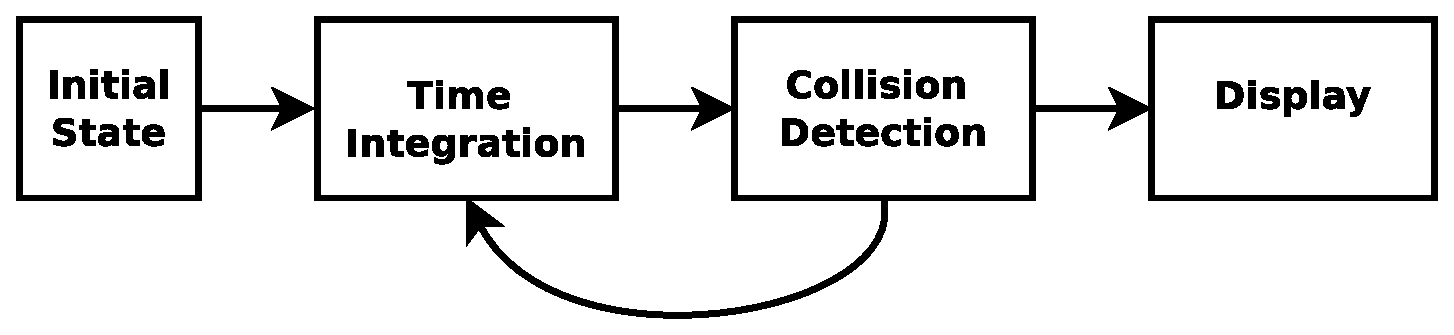
\includegraphics[width=.95\textwidth]{simulation_pipeline3.eps}}
            \only<3>{ 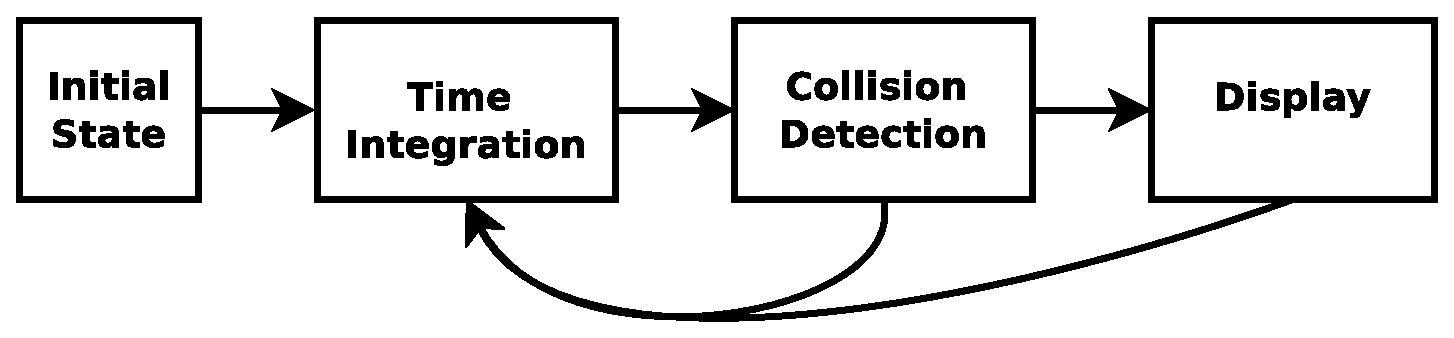
\includegraphics[width=.95\textwidth]{simulation_pipeline4.eps}}
            \only<4->{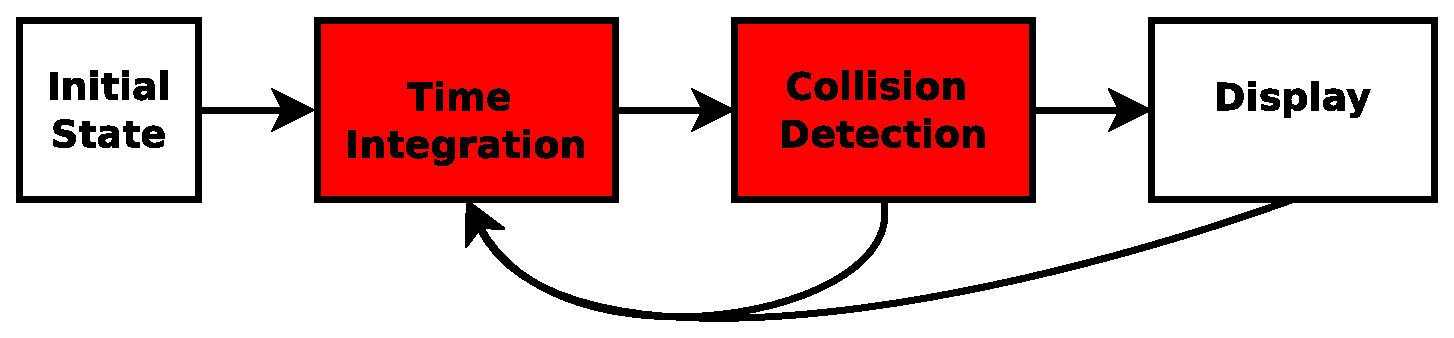
\includegraphics[width=.95\textwidth]{simulation_pipeline5.eps}}
        }
    \end{block}
    \pause
    \pause
    \pause
    \pause
    \begin{exampleblock}{Sofa \cite{Allard07SOFA,Nesme09Preserving,Faure11Sparse}}
        \begin{columns}
            \column{.5\textwidth}
            \begin{itemize}
                \item<5-> Scientific purpose: \alert<5-6>{Precise}
                \item<6-> Surgery training: \alert<6>{Interactive} 
                \item<8-> \alert<8>{Abstract} Framework
                    \begin{itemize}
                        \item Highly modular
                        \item Deep class tree
                    \end{itemize}
            \end{itemize}
            \column{.5\textwidth}
            \begin{itemize}
                \item<7-|alert@+-> High performances
                    \vspace{.7cm}
                \item<9-|alert@+-> Require profiling
            \end{itemize}
        \end{columns}
    \end{exampleblock}
\end{frame}

\begin{frame}{Previous parallelization of Sofa}
    \begin{itemize}[<+->]
        \item Everton Hermann \cite{Hermann10Simulations} \\
            \begin{itemize}
                \item Parallelization between objects using Kaapi
                \item Good speedup (15 using 16 CPUs), better with GPUs
                \item Not used in recent Sofa version 
            \end{itemize}
        \item Julio Toss \cite{Toss12New}
            \begin{itemize}
                \item Works on algorithms out of Sofa then incorporate them
                \item Ongoing work
            \end{itemize}
        \item Current version openmp \#pragma for
            \begin{itemize}
                \item Sometimes better results without openmp
                \item No previous analysis
            \end{itemize}
    \end{itemize}
    \uncover<11>
    {
        \begin{alertblock}{Limits}
            \begin{itemize}
                \item Parallelization of small parts of Sofa
                \item Bottlenecks are not clearly identified
            \end{itemize}
        \end{alertblock}
    }
\end{frame}
\begin{frame}{Parallelization and scheduling schemes within Sofa}
    \pause
    \begin{block}{Approach}
        \begin{itemize}
            \item Focus on Sofa 
            \item Identify performance issues
            \item Find Parts of code which can be improved
            \item Without going directly deep on the code 
        \end{itemize}
    \end{block}
    \pause
    \begin{alertblock}{Objectives (long term)}
        Describe a reproducible methodology to optimize complex applications
    \end{alertblock}
\end{frame}


\newsection{Analysis}

\begin{frame}{First Analysis}
    \begin{block}{Questions}
        \begin{itemize}
            \item What are we looking for ?
            \item How can we identify it ?
            \item What kind of tools should we use ?
            \item What metrics are relevants ?
        \end{itemize}
    \end{block}
    \pause
    \begin{alertblock}{Idea}
        Use performance counter for an overview exploration
    \end{alertblock}
    \pause
    \begin{exampleblock}{Challenges}
        \begin{itemize}
            \item Lot of data
            \item How to correlate different metrics ?
        \end{itemize}
    \end{exampleblock}
 %   \begin{block}{Methodology}
 %       \begin{itemize}
 %           \item Performances counter using Likwid \cite{Treibig10LIKWID}
 %           \item Analysis at a global level (wrapper mode)
 %           \item Analysis at a local level (marker mode)
 %           \item Counters for all cache level, memory, Cycles per instructions
 %           \item Performance metrics from Sofa (Simulation time, FPS)
 %           \item 4 representative scenes
 %       \end{itemize}
 %   \end{block}
 %   \pause
 %   \begin{exampleblock}{First results}
 %       \begin{itemize}
 %           \item Hundred of plots
 %           \item Lot of work to correlate them / keep only the interesting ones
 %       \end{itemize}
 %   \end{exampleblock}
\end{frame}

\begin{frame}{Results}

    \only<1-2>{\includegraphics[width=0.9\textwidth]{img/Runtime_ratio1.png}}
    \only<3-4>{\includegraphics[width=.9\textwidth]{img/memory_traffic_loc2.png}}
    \only<5->{\includegraphics[width=.9\textwidth]{img/memory_traffic_loc1.png}}
    \begin{textblock}{14}(1,5)
        \only<2>{
            \begin{block}{Observations}
                \begin{itemize}
                    \item ApplyJ and ApplyJT vec represent an important part
                        of the execution
                    \item The speedup is only about 2 with 4 cores
                    \item High CPI (not shown here)
                        \begin{itemize}
                            \item Wrong prediction (pipeline not fill)
                            \item Bad memory use
                        \end{itemize}
                    \item A significative part of the simulation is missing
                \end{itemize}
            \end{block}
        }
        \only<4>{
            \begin{block}{Observations}
                \begin{itemize}
                    \item ApplyJ and ApplyJT vec uses a lot of L2 cache
                    \item The amount of data doesn't change for openmp version
                    \item Memory seems to be shared between threads
                \end{itemize}
            \end{block}
        }
        \only<6->
        {
            \begin{alertblock}{First conclusions}
                \begin{itemize}
                    \item High use of L2 (private) cache
                    \item Low bandwith
                    \item High CPI 
                    \item Maybe a problem of false sharing
                    \item We need more informations
                        \begin{itemize}
                            \item Memory use by threads 
                            \item Memory access patterns
                        \end{itemize}

                \end{itemize}
            \end{alertblock}
        }
    \end{textblock}
\end{frame}

\begin{frame}{Other tools}
    \begin{block}{CPU oriented}
        \begin{columns}
            \column{.51\textwidth}
            \begin{itemize}
                \item PAPI \cite{Weaver13PAPI}
                \item Oprofile \cite{Oprofile}
                \item Vtunes \cite{Reinders05VTune}
                \item \dots
            \end{itemize}
            \column{.35\textwidth}
            \begin{alertblock}{Limits}
                Answer the same questions
            \end{alertblock}
        \end{columns}
    \end{block}
    \uncover<2->
    {
        \begin{block}{Others}
            \begin{columns}
                \column{.6\textwidth}
                \begin{itemize}
                    \item HPCToolkit \cite{Adhianto10HPCTOOLKIT}
                    \item Paraver \cite{Pillet95PARAVER}
                    \item MemProf \cite{Lachaize12MemProf}
                \end{itemize}
                \column{.25\textwidth}
                \begin{alertblock}{Limits}
                    Answer other questions \\but not the one we asked
                \end{alertblock}
            \end{columns}

        \end{block}
    }
\end{frame}
\newsection{Current work and perspective}

\begin{frame}{Designing new tool}
    \begin{itemize}
        \item Detect patterns
            \begin{itemize}
                \item Dispersion between structures
                \item Dispersion inside a structure
                \item Frequency
                \item Linearity
            \end{itemize}
        \item Detect sharing
            \begin{itemize}
                \item Concurrent access
                \item Shared structures
            \end{itemize}
    \end{itemize}
\end{frame}
\begin{frame}{Heapinfo \cite{Beniamine13Cartographier}}
    \begin{figure}
        \centering
        \includegraphics[width=.65\linewidth]{img/mat_naif_50_42_0_none_naif.pdf}
    \end{figure}
\end{frame}

\newcounter{finalframe}
\setcounter{finalframe}{\value{framenumber}}
%Last numbered frame go here
\begin{frame}{Perspectives}
    \begin{itemize}
        \item Instrumentation is slow
            \begin{itemize}
                \item Other methods ?
                \item Larger grain ?
            \end{itemize}
        \item Lot of data
            \begin{itemize}
                \item How can we analyse them ?
                \item What are the relevAnt metrics ?
                \item How can we visualize them ? 
            \end{itemize}
    \end{itemize}
\end{frame}

%=============================================================================

%=============================================================================
%Uncomment next lines for uncounted backup slides & biblio
\newHsection{Bibliography}
\setboolean{sectiontoc}{false} 
%
\bibliographystyle{apalike} 
\bibliography{presentation}

%========================= Backup slides =====================================
%\newsection*{Hidden slides}
%put this line before each frame
%\setcounter{framenumber}{\value{finalframe}}

%=============================================================================
\end{document}


